% !TEX root = ../slides.tex

\section{Background on APN functions}
\begin{frame}
	\frametitle{Vectorial Boolean functions}
\vspace{-20pt}
 $$\cF \from \FF_2^\cn \to \FF_2^{\green{n}}$$
 \pause
\vspace{-20pt}
\begin{mybox}[cblue]{Representations}
\begin{itemize}
	\item[-] Multivariate $\cF = (\cF_1, \dotsc, \cF_\green{n})$ where $\cF_i \from \FF_2^{\cn} \to \FF_2$ \hfill \green{n} coordinates in $\cn$ variables ($\FF_2$)
	\item[-] Univariate: (up to identification) $\cF \from \FF_{2^\cn} \to \FF_{2^\green{n}}$ \hfill 1 coordinate, 1 variable ($\FF_{2^\cn}$)
\end{itemize}
\end{mybox}

\pause
\begin{mybox}[corange]{Every function is polynomial}
\begin{itemize}
	\item[-] Multivariate degree $\max_{i = 1,\dotsc,\green{n}}(\deg(\cF_i))$
	\item[-] Univariate degree $\deg(\cF)$
	\item[-] Linear, quadratic\dots refer to \orange{multivariate}
\end{itemize}
\end{mybox}
\pause
\begin{mybox}[cgreen]{}
$\cF \from \FF_{2^{\brown{6}}} \to \FF_{2^{\green{6}}}, X \mapsto X^3 + X^{10} + uX^{24}$ \hfill $\deg(\cF) = 24$
\vspace{10pt}

\only<5>{
$\cF_1 = x_1x_4 + x_1x_5 + x_2x_3 + x_2x_6 + x_3 + x_4x_5 + x_4x_6 + x_4 + x_5$ \hfill$\deg(\cF_1) = 2$

$ \ \vdots$

$\cF_6 = x_1x_2 + x_1x_4 + x_2x_4 + x_2x_5 + x_2 + x_3x_4 + x_3x_6 + x_4 + x_5x_6 + x_6$ \hfill$\deg(\cF_6) = 2$
}


\onslide<6->{$\cF$ is quadratic}
\onslide<7->{\hfill 3 = 0b0000\red{11}, 10 = 0b00\red{1}0\red{1}0, 24 = 0b0\red{11}000}

\end{mybox}

\end{frame}


\begin{frame}
	\frametitle{APN functions}
\vspace{-10pt}
 $$\forall \calpha, \cbeta, \quad \delta_{\cF}(\calpha, \cbeta) \vcentcolon= \card{\set{x \in \FF_{2^\cn}, \  \cF(x + \calpha) + \cF(x) = \cbeta }}$$
 \pause
\vspace{-10pt}
\begin{mybox}[cblue]{Differential uniformity}
The differential uniformity of $\cF$ is $\Delta_{\cF} \vcentcolon= \max_{\alpha\neq 0, \beta} \delta_{\cF}(\calpha, \cbeta)$. 

\vspace{5pt}
A function is \blue{Almost Perfect Non-linear} (APN) if $\Delta_{\cF} = 2$.
\end{mybox}

\pause
\begin{mybox}[corange]{The linear case}
$\cF$ linear.
$$ \cF(x + \calpha) + \cF(x) \quad  = \quad \cF(x) + \cF(\calpha) + \cF(x) \quad  = \quad \cF(\calpha)$$

$\calpha \neq 0$. $\quad \quad \delta_{\cF}(\calpha, \cbeta) = \left\{
    \begin{array}{ll}
        2^{\cn} & \text{ if } \cbeta = \cF(\calpha)\\
        0 & \text{ otherwise.}
    \end{array}
\right.$
\end{mybox}
\pause
\begin{mybox}[cgreen]{The APN case}
$\cF$ APN. Then $ \forall \ \calpha\neq 0, \quad \card{\set{\cbeta, \ \ \delta_{\cF}(\calpha, \cbeta) > 0 }} = 2^{n-1}$.
\end{mybox}

\end{frame}


\begin{frame}
	\frametitle{Equivalence relations}
	\vspace{-10pt}
\recapbox{
$ \cF, \redG \from \FF_2^\cn \to \FF_2^\cn, \quad \quad \graphF =  \set{\begin{pmatrix}
x\\
\cF(x)
\end{pmatrix}, x \in \FF_{2^n}}, \quad \quad \graphG =  \set{\begin{pmatrix}
x\\
\redG(x)
\end{pmatrix}, x \in \FF_{2^n}}$}
\pause
\begin{mybox}[cblue]{Affine equivalence}
 $\cF \sim_{A} \redG \ \iff \ \exists \ \cA, \cB \quad  \cA \comp \cF \comp \cB = \redG \quad \iff \quad  \begin{pmatrix}
\cB^{-1} & 0\\
0 & \cA 
\end{pmatrix}\graphF= \graphG$ 
\vspace{5pt}

with $\cA, \cB$ affine, bijective.
\end{mybox}

\pause
\begin{mybox}[cblue]{Extended-affine equivalence}
 $\cF \ea \redG \ \iff \ \exists \ \cA, \cB, \cC \quad  \cA \comp \cF \comp \cB + \cC = \redG \quad \iff \quad  \begin{pmatrix}
\cB^{-1} & 0\\
\cC\cB^{-1} & \cA 
\end{pmatrix}\graphF= \graphG$ 
\vspace{5pt}

with $\cA, \cB, \cC$ affine, $\cA, \cB$ bijective.
\end{mybox}
\pause

\begin{mybox}[cblue]{CCZ equivalence}
 $\cF \ccz \redG \ \iff \ \exists \ \ccalA \text{ affine, bijective } \quad  \ccalA(\graphF) = \graphG$. \hfill $\ccalA = \ccalL + \cc$
\end{mybox}
\end{frame}

\begin{frame}
\frametitle{CCZ equivalence and differential properties}
\vfill
\recapbox{$\cF \ea \redG \ \iff \ \exists \ \cA, \cB, \cC \quad  \cA \comp \cF \comp \cB + \cC = \redG$

$\cF \ccz \redG \ \iff \ \exists \ \ccalA \text{ affine, bijective } \quad  \ccalA(\graphF) = \graphG$. \hfill $\ccalA = \ccalL + \cc$}
\begin{mybox}[cblue]{Example}
Let $\cF \from \FF_{2^{\cn}} \to \FF_{2^{\cn}}$ bijective. Then $\cF \ccz \cF^{-1}$.

$\mathcal{G}_{\cF^{-1}} = \begin{pmatrix}
0 & \mathrm{Id}\\
\mathrm{Id} & 0 
\end{pmatrix} \graphF $
\end{mybox}
\pause
\begin{mybox}[cgreen]{Main usage of CCZ equivalence}
Let $\cF \ccz \redG$. $\quad$
Then $\ \ \forall \ \calpha,\cbeta, \quad  \delta_{\redG}(\calpha, \cbeta) = \delta_{\cF}(\ccalL^{-1}(\calpha, \cbeta))$. 
\end{mybox}
\pause
\begin{mybox}[cred]{Invariants}
 $\cF \ccz \redG \quad \implies \quad \duF = \duG$.
\vspace{3pt}

 $\cF \ccz \redG \ \centernot\implies \ \mathrm{multideg}(\cF) = \mathrm{multideg}(\redG)$.
\vspace{3pt}

But $ \cF \ea \redG \  \implies \ \mathrm{multideg}(\cF) = \mathrm{multideg}(\redG).$
 \end{mybox}

\end{frame}



\begin{frame}
	\frametitle{Known APN constructions}
	\begin{chronology}[5]{1992}{2024}{15cm}[\textwidth]
\eventpoint{1992}{ \ \ [NybKnu92]}[cblue][1][1]
\eventpoint{1993}{ \ \ [Nyberg93]}[cblue][1][1]
\eventspan{1992}{2001}{}[cgreen][.5][.2]
\eventpoint{2006}{ \ \ [BCP06, EKP06]}[cblue][1][1]
\eventspan{2006}{2024}{}[cred][.5][.2]
\end{chronology}
\vspace{20pt}
\begin{itemize} 
	\item[-] \blue{1992}: APN definition \hfill [NybKnu92]% Provable Security Against Differential Cryptanalysis
	\item[-] \blue{1993}: First APN power mappings $x \mapsto x^{2^i + 1}$\hfill [Nyberg93]% Provable Security Against Differential Cryptanalysis
	\item[-] \green{1993-2001}: 5 more families of APN non-quadratic \green{power mappings}% Provable Security Against Differential Cryptanalysis
	\pause
	\vspace{10pt}
	\item[-] \blue{2006}: First APN functions CCZ-inequivalent to a power function. \hfill [BCP06, EKP06] %Budaghyan, Carlet \& Pott 2006 A. New classes of almost bent and almost perfect nonlinear polynomials.
	\item[-] \red{2007-2024} : $\simeq 20$ infinite families of \red{quadratic} APN functions.
\end{itemize}
\end{frame}

\begin{frame}
	\frametitle{LOTS of open questions}


\begin{mybox}[cblue]{Two major classes}
\begin{itemize}
	\item[1)] \green{Power mappings} $x \mapsto x^d$
	\item[2)] \red{Quadratic} functions
\end{itemize}
All known APN functions are CCZ-equiv to 1) or 2) \ \ \ \dots \ \orange{except one}.
\end{mybox}

\begin{mybox}[corange]{}
More APN functions CCZ-\orange{inequivalent} to monomials and quadratic functions? 
\end{mybox}
\pause
\vspace{15pt}
\begin{mybox}[cblue]{APN bijections}
\begin{itemize}
	\item[-] Some are known for odd $\cn$ \hfill (e.g. APN powers)
	\item[-] None are known for even $\cn$ \ \ \ \dots \ \red{except one}.
\end{itemize}
\end{mybox}

\begin{mybox}[cred]{}
\red{Big APN problem}: More APN bijections in \red{even} dimension ? 
\end{mybox}

\end{frame}


\begin{frame}
	\frametitle{Zoo of APN functions}
	\vfill
	\includegraphics[scale=.28]{figures/table_1}
	\includegraphics[scale=.28]{figures/table_2}


\only<2>{
	\begin{textblock*}{7cm}(3cm,3.5cm)
\begin{tcolorbox}[colback=cred!5!white,colframe=cred]
\red{Relationships between each others?}
\end{tcolorbox}
\end{textblock*}

	\begin{textblock*}{7cm}(6cm,6.5cm)
\begin{tcolorbox}[colback=cred!5!white,colframe=cred]
\red{Is this classification that wide?}
\end{tcolorbox}
\end{textblock*}
}

\end{frame}


\section{Cryptanalysis of the Kim mapping}
\begin{frame}
	\frametitle{The (only ?) solution to the big APN problem}

\begin{mybox}[cred]{Big APN problem}
Does there exist an APN bijection in \red{even} dimension ? 
\end{mybox}

\begin{mybox}[cblue]{Known facts \hfill [Hou06]}
An APN bijection for $\cn = 2t$
\begin{itemize}
	\item[-] does not exist for $\cn \in \set{2, 4}$
	\item[-] cannot be quadratic
	%\item[-] cannot be a polynomial with coefficients in $\FF_{2^k}$.
\end{itemize}

\end{mybox}
\pause
\vspace{-10pt}
  \begin{columns}[T]
    \begin{column}{0.45\textwidth}
      \begin{mybox}[cblue]{Kim mapping}
        \begin{equation*}
          \kim :
          \begin{cases}
            \FF_{2^{\red{6}}} &\to \FF_{2^{\red{6}}} \\
            x &\mapsto x^3 + x^{10} + u x^{24}
          \end{cases}
        \end{equation*}

        APN, quadratic, \red{not} bijective
      \end{mybox}
    \end{column}
    \pause
    \begin{column}{0.09\textwidth}
    \vspace{20pt}
      \begin{center}
      $\not\sim_{EA}$
\pause

      \vspace{10pt}
        $\ccz$

        
      \end{center}
    \end{column}
    \begin{column}{0.45\textwidth}
      \begin{mybox}[cred]{Dillon et al.'s permutation }
        \begin{equation*}
          P :
          \begin{cases}
            \FF_{2^{\red{6}}} &\to \FF_{2^{\red{6}}} \\
            x &\mapsto P(x)
          \end{cases}
        \end{equation*}

        APN, \red{not} quadratic, \red{bijective}
      \end{mybox}
    \end{column}
  \end{columns}
  \hfill [BDMW10]
\end{frame}

\begin{frame}
\frametitle{Walsh transform}
    
\begin{mybox}[cblue]{Walsh transform}

$\cF \from \FF_{2^\cn} \to \FF_{2^\cn} $. $\calpha, \cbeta \in \FF_{2^\cn}.$

$$ \cFh(\calpha, \cbeta) \vcentcolon= \sum_{x \in \FF_{2^\cn}} (-1)^{\calpha\cdot x + \cbeta\cdot F(x)}$$
\end{mybox}

\pause
\begin{mybox}[cgreen]{Walsh transform and CCZ-equivalence}

$\cF, \redG \from \FF_{2^\cn} \to \FF_{2^\cn} $.
\vspace{5pt}

$\ccalA = \ccalL + \cc \quad \quad \ccalA(\graphF) = \graphG \quad \quad \iff \quad \quad \widehat{\redG}(\calpha, \cbeta) = (-1)^{c\cdot(\calpha, \cbeta)} \cFh(\ccalL^\top (\calpha, \cbeta)) \quad \forall \calpha,\cbeta \in \FF_{2^\cn}$
\end{mybox}

\end{frame}



\begin{frame}
	\frametitle{A cryptanalytic point of view}
\vspace{-15pt}
\recapbox{$\cF, \redG \from \FF_{2^\cn} \to \FF_{2^\cn} \hfill \cFh(\calpha, \cbeta) \vcentcolon= \sum_{x \in \FF_{2^\cn}} (-1)^{\calpha\cdot x + \cbeta\cdot F(x)}$.
\vspace{5pt}

$\ccalA = \ccalL + \cc \quad \quad \ccalA(\graphF) = \graphG \quad \quad \iff \quad \quad \widehat{\redG}(\calpha, \cbeta) = (-1)^{c\cdot(\calpha, \cbeta)} \cFh(\ccalL^\top (\calpha, \cbeta)) \quad \forall \calpha,\cbeta \in \FF_{2^\cn}$
}
\pause
\vspace{-5pt}

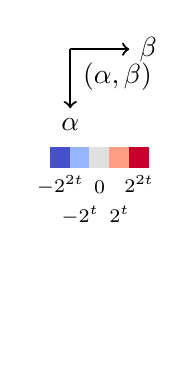
\begin{tikzpicture}[scale=.25]
\draw[->,thick] (0,0)--(3,0) node[right]{$\beta$};
\draw[->,thick] (0,0)--(0,-3) node[below]{$\alpha$};
\node at (2.4, -1.4) { $\cFh(\alpha, \beta)$};
\draw[transparent] (0, -15) rectangle (1, 1) ;

\definecolor{orangeLAT}{HTML}{fe9e82}
\definecolor{redLAT}{HTML}{c7002c}
\definecolor{lightblueLAT}{HTML}{96b6ff}
\definecolor{blueLAT}{HTML}{4851cc}
\definecolor{greyLAT}{HTML}{e1e0e0}


\draw[blueLAT, fill=blueLAT] (-1, -6) rectangle node[below=3] {\scriptsize \color{black} ${-2}^{2t}$} (0, -5);
\draw[lightblueLAT, fill=lightblueLAT] (0, -6) rectangle node[below=14] {\scriptsize \color{black} ${-2}^t$} (1, -5);
\draw[greyLAT, fill=greyLAT] (1, -6) rectangle node[below=5] {\scriptsize \color{black} $0$} (2, -5);
\draw[orangeLAT, fill=orangeLAT] (2, -6) rectangle node[below=14] {\scriptsize \color{black} $2^t$} (3, -5);
\draw[redLAT, fill=redLAT] (3, -6) rectangle node[below=3] {\scriptsize \color{black} $2^{2t}$} (4, -5);
\end{tikzpicture}
\includegraphics[scale=.098]{figures/dillon_lat}
%\begin{overpic}[scale=.098]{figures/dillon_lat}
          %\begin{tikzpicture}[scale=6.5]
           % \draw[transparent] (0, 0) rectangle (1, 1) ;
            % \onslide<2->{
            %   \draw[ForestGreen, line width=.5mm] (0.1mm, 0) -- +(0, 1);
            %   }
            % \onslide<3->{
            %   \draw[ForestGreen, line width=.5mm] (0, 0.945) -- +(.97, 0);
            % }
          %\end{tikzpicture}
        %\end{overpic}
\only<4->{
\begin{textblock*}{10cm}(11cm,9.35cm)
Kim mapping
\end{textblock*}
}
\only<3>{ \begin{textblock*}{10cm}(9.8cm,4.5cm)
$\cFh ({\set{0} \times \FF_{2^\cn}^*}) = \set{0} $.
\vspace{10pt}

$\cFh ({\FF_{2^\cn}^*} \times \set{0}) = \set{0} $.
\vspace{10pt}

$ {\FF_{2^\cn}} \times \set{0} \ \bigcap  \ \set{0} \times {\FF_{2^\cn}} = \set{0}$
\vspace{10pt}

$\mathcal{L}^\top $linear bijection.
\end{textblock*}}
\only<4>{
\includegraphics[scale=.098]{figures/kim_lat_unsorted}
}
\only<5->{
\includegraphics[scale=.097]{figures/kim_lat}	
}
\only<2->{
\begin{textblock*}{10cm}(4cm,9.35cm)
Dillon APN bijection
\end{textblock*}}

% \begin{textblock*}{5cm}(9.2cm,7.8cm)
% Cube over $\FF_{64}$ $x \mapsto x^3$
% \end{textblock*}



\end{frame}


